\documentclass[letterpaper,twocolumn,10pt]{article}
\usepackage{usenix,epsfig,endnotes,amsmath}
\usepackage{graphicx}
\begin{document}

\date{}

\title{\Large \bf Real-Time Detection of Lateral Movement in Cloud VPC Networks via Graph-Based Analysis of Flow and Authentication Logs}

\author{
{\rm Ibrahim Pehlivan}\\
University of California, Los Angeles
\and
{\rm Wesley Gunawan}\\
University of California, Los Angeles
\and
{\rm Samyak Kakatur}\\
University of California, Los Angeles
}

\maketitle

\thispagestyle{empty}


\subsection*{Abstract}
Lateral movement in cloud VPC networks is notoriously difficult to detect because internal traffic is trusted by default and no single log source provides complete visibility into attacker behavior. We present a graph-based detection system that combines network flow logs and authentication logs into a unified streaming graph, extracts structural, temporal, and statistical features, and scores nodes and edges for lateral movement likelihood. Our evaluation on the LANL-Dataset-2015 (58 days, 1.6B+ events, 749 labeled red-team attacks) and DAPT2020 (simulated APT with labeled kill-chain stages) demonstrates that the combined method achieves the highest AUC (0.9456) and lowest false positive rate (0.0005) compared to single-source baselines. We identify three key detection signals: attack traffic is overwhelmingly TCP (99.82\% vs. 50\% benign), the fan-out ratio follows a predictable arc across the kill chain (2.5 $\rightarrow$ 6.0 $\rightarrow$ 1.0), and attackers exhibit 35.7$\times$ longer inter-arrival times than normal users. Feature importance analysis reveals that active duration (5.5$\times$ higher for attackers), inter-arrival variance (4.5$\times$), and in-degree (3.3$\times$) are the strongest discriminators. These findings confirm that multi-log graph analysis provides richer detection signal than single-source methods, though low pair-space recall highlights the challenge of isolating rare attack edges in massive enterprise graphs.

\section{Introduction}

Cloud VPC networks present a complex security landscape where internal traffic flows freely between hosts by default. Lateral movement, the phase of an attack where an adversary pivots through a compromised network to reach high-value targets, is especially difficult to detect because the volume of benign connections dwarfs the few that matter. Existing intrusion detection tools were built for perimeter monitoring and struggle with the noise and dynamism of cloud VPC environments, where diverse user activity and constant connection churn mask attacker activity.

No single log source provides enough signal to reliably identify lateral movement. Network flow logs capture connections but cannot distinguish an attacker's session from an admin's; authentication logs record login events but are blind to reconnaissance via port scans or data exfiltration that never triggers a login. Prior detection methods have relied on either signature matching, which misses novel attack patterns, or anomaly detection on a single log source, which floods analysts with false positives on busy production networks. We propose combining both log types into a unified streaming graph where computers and identities are nodes, connections and authentication events are edges, and graph-based feature analysis can detect the structural and temporal patterns that distinguish lateral movement from routine operations. This paper presents our graph construction pipeline, the detection methodology, and an evaluation on the LANL-Dataset-2015 and DAPT2020 datasets against single-source baselines.

\section{Related Work}

Graph-based detection methods model relationships between system events and reason over paths or substructures. Hopper~\cite{hopper2021} builds a login graph from authentication events and uses path inference to flag lateral movement sequences. However, its reliance on authentication logs alone means it cannot detect movement that bypasses login entirely, such as exploitation of services or use of stolen session tokens. We extend this idea by incorporating network flow logs, capturing lateral movement paths that never produce an authentication event. Euler~\cite{euler2023} applies temporal link prediction to cloud VPC network graphs, treating lateral movement as a link prediction problem in an evolving graph. Its temporal modeling is a strong baseline for our own temporal graph features, though it operates on a single data source. POIROT~\cite{poirot2019} matches provenance graph templates against audit logs to detect known attack patterns. Template matching is effective when attack structures are known in advance but cannot catch novel variations; we use anomaly-based scoring instead and adapt the graph model to cloud VPC network logs rather than host-level audit data.

Multi-log correlation approaches combine evidence from separate data sources to improve detection coverage. HOLMES~\cite{holmes2019} correlates system audit logs across multiple stages of the kill chain, mapping observed behavior to MITRE ATT\&CK tactics and producing a real-time threat score. Its multi-stage correlation confirms that combining log sources can improve detection, and its kill-chain framing shaped our detection pipeline structure. However, HOLMES operates on host-level audit logs in traditional enterprise settings, whereas we target network flow logs and authentication events at cloud VPC network scale.

\section{Background and Problem Setting}
\begin{itemize}
\item Lateral movement definition: post-exploitation phase where attacker pivots through network to reach targets, sits between initial access and objectives (data exfiltration, privilege escalation)
\item Kill-chain context: reconnaissance, initial compromise, lateral movement, objective completion
\item Cloud VPC architecture: virtual private cloud with VMs, subnets, firewall rules; VPC flow logs record source/dest IP, ports, bytes, packets; cloud audit/auth logs record SSH attempts, service account usage, IAM events
\item Threat model: assumes one computer already compromised (e.g., via phishing or vulnerable service); attacker goals include reaching high-value targets, expanding access via credential reuse, exfiltrating data; attacker capabilities include port scanning, SMB lateral movement, credential stuffing, service exploitation; red-team ground truth provides labeled attack events
\item Why existing tools fall short: perimeter IDS sees only north-south traffic; host-based agents miss network context; SIEM correlation rules are brittle and require manual tuning; network flow analysis alone lacks authentication context
\end{itemize}

\section{Methods and Approach}

We test whether a graph built from both network flow and authentication logs detects more red-team lateral movement pairs than graphs from either source alone. We also run five unsupervised anomaly detectors on the same edge feature matrix to check whether hand-crafted scoring outperforms generic tabular methods.

\subsection{Graph Construction}

We model the network as a directed multigraph in igraph. Nodes are computers and users; edges are authentication events or network flows. A \texttt{StreamingGraphBuilder} reads gzipped CSV files line-by-line, keeping only events within merged time windows derived from red-team ground truth (Section~5.1). Events outside all windows are skipped, so memory stays proportional to active windows, not the full 1.6-billion-event dataset.

For each authentication event, the builder adds a computer-to-computer edge storing auth type, logon type, orientation, success, and timestamp. If both source and destination users are present, a user-to-user edge is added with the same attributes. For each flow event, a computer-to-computer edge stores protocol, source/destination ports, packet count, byte count, duration, and timestamp. When multiple events share the same $(src, dst)$ pair, the edge weight increments and only the first and last timestamps are kept. Duplicates become weight, not separate edges. Node types are inferred by a simple rule: names containing \texttt{\$} before \texttt{@} or ending with \texttt{\$} are machine accounts; everything else is a user.

After all events are streamed, the edge map is materialized into an igraph object. Three graph variants are built per run: \emph{flow-only} ($\approx$11,586 nodes, 131,562 edges), \emph{auth-only} ($\approx$90,783 nodes, 409,100 edges), and \emph{combined} ($\approx$91,589 nodes, 512,529 edges). Each graph is freed after scoring to limit memory to roughly 4~GB.

\subsection{Feature Extraction}

We extract features at three levels (node, edge, graph) independently for each variant.

\textbf{Node features.}
For each node we compute in-degree, out-degree, total degree, and fan-out ratio (out-degree / total degree). Fan-out ratio targets a specific lateral movement pattern: compromised hosts performing reconnaissance connect to many distinct destinations (high fan-out), while normal servers mostly receive connections (low fan-out). Betweenness centrality is computed exactly for graphs under 5,000 nodes; for larger graphs we use igraph's cutoff parameter at 3~hops, which approximates betweenness in $O(|E|)$ instead of $O(|V||E|)$.

We also compute four temporal features per node from the timestamps of its outgoing edges: mean and standard deviation of inter-arrival times, a burst score (maximum fraction of outgoing edges falling within any 10\% sub-window of the node's active span), and total active duration. The burst score separates reconnaissance, which produces many connections in a short burst, from persistent movement, which has longer and more regular spacing.

\textbf{Edge features.}
Each edge receives 12 features. For all edges: edge rarity ($1 / \text{weight}$), source out-degree, destination in-degree, source fan-out, normalized weight, self-loop flag, and user-edge flag. For authentication edges specifically: whether the auth type is NTLM, whether the logon type is Network (remote access), and whether authentication succeeded. For flow edges specifically: whether the destination port is in the lateral movement set $\{$22, 23, 445, 3389, 5985, 5986$\}$ or above 49,152 (ephemeral); protocol rarity ($1 - \text{proportion of edges using that protocol}$); byte-per-packet ratio as a percentile rank; and duration z-score. Self-loops and user-to-user edges are excluded from scoring.

\textbf{Graph features.}
Density, average clustering coefficient (computed on the undirected version), weakly connected component count, node count, and edge count.

\subsection{Edge Scoring}

Edges are scored with a weighted sum whose terms depend on edge type. The weights are set from domain knowledge (NTLM is common in pass-the-hash attacks, uncommon connections are more suspicious) and have not been tuned; we plan to optimize them in future work.

Authentication edges:
\begin{equation}
\begin{aligned}
s_{\text{auth}} ={}& 0.4 \cdot \text{is\_ntlm} \\
                  &+ 0.3 \cdot \text{is\_network\_logon} \\
                  &+ 0.3 \cdot \text{rarity\_rank}
\end{aligned}
\end{equation}
NTLM gets the highest weight because pass-the-hash attacks produce NTLM authentication events on networks that predominantly use Kerberos. Network logon type indicates remote access. Rarity rank is the percentile of $1/\text{weight}$ among all edges: low-weight edges are unusual and thus more suspicious.

Flow edges:
\begin{equation}
\begin{aligned}
s_{\text{flow}} ={}& 0.4 \cdot \text{rarity\_rank} \\
                  &+ 0.3 \cdot \text{is\_unusual\_dst\_port} \\
                  &+ 0.3 \cdot \text{protocol\_rarity\_rank}
\end{aligned}
\end{equation}
Rarity is weighted highest because uncommon source-destination pairs are the strongest single signal in flow data. The unusual-port flag encodes knowledge of which services attackers use for lateral movement. Protocol rarity captures deviations from the normal protocol distribution.

For the combined method, auth edges receive a $1.5\times$ multiplier because auth signals are more informative per edge but far fewer in number (409k auth edges vs.\ 131k flow edges). Without this multiplier, auth scores would be drowned out by the larger flow population.

\subsection{Path Scoring}

Single-edge scoring misses multi-hop attack chains. To capture these, we enumerate paths through the graph via breadth-first search from every node, up to 4~hops, following only the top 10 outgoing edges per node ranked by edge score. Enumeration runs in parallel across 12 CPU workers.

Each path is scored as the mean of three aggregates of its constituent edge scores: geometric mean (high if every edge is somewhat suspicious), maximum edge score (high if any single hop is very suspicious), and arithmetic mean. The top 50 paths by score are retained. Every edge that appears in a top-50 path receives a boost of $0.1 \times \text{path\_score}$ added to its own score, capped at 1.0. This feeds path-level signal back into edge-level detection.

\subsection{Unsupervised Baselines}

We also run five unsupervised anomaly detectors on the 12-dimensional edge feature vector: Isolation Forest (100 trees, 5\% contamination), Local Outlier Factor, One-Class SVM (RBF kernel, $\nu{=}0.1$), Elliptic Envelope, and PCA reconstruction error. Each detector is trained on benign edges only and produces an anomaly score for every edge. This gives a direct comparison between hand-crafted scoring and standard learned methods on the same ground-truth pairs. All five use scikit-learn defaults except where noted.

\subsection{Threshold Selection}

Anomalous edges are identified by thresholding final edge scores. We sweep percentiles $[90, 95, 97, 99, 99.5, 99.9]$ and pick the one that maximizes F1 against known red-team pairs. The selected thresholds are 95th percentile for auth-only, 97th for flow-only, and 97th for combined. We acknowledge that optimizing on the same labeled data used for evaluation is a limitation: these thresholds may not generalize to unseen attack patterns.

\section{Data and Experimental Setup}

\subsection{Datasets}

\textbf{LANL Cybersecurity Dataset (LANL-2015).}
The primary dataset is the Los Alamos National Laboratory cybersecurity dataset~\cite{kent-2015-cyberdata1}, covering 58 days of continuous network activity. It contains approximately 1.6 billion events across 12,425 users and 17,684 computers in three gzipped CSV files: \texttt{auth.txt.gz} (authentication events with timestamp, source/destination users and computers, auth type, logon type, orientation, success/failure), \texttt{flows.txt.gz} (network flow events with timestamp, duration, source/destination computers and ports, protocol, packet count, byte count), and \texttt{redteam.txt.gz} (749 labeled red-team attack events forming 308 unique source-destination pairs). Red-team events include lateral movement via SMB, SSH, RDP, credential reuse, and network reconnaissance; 93.6\% originate from a single compromised host (C17693) used as a jump box.

Because loading 1.6 billion events is impractical, we scope the data using time windows. For each red-team event, we define a window of $\pm$3,600 seconds. Overlapping windows are merged, producing 25 non-overlapping intervals that capture approximately 104 million auth events and 31.6 million flow events. Events are streamed directly from the gzipped files: only events falling inside a window are parsed, and parsing stops once the timestamp exceeds the last window.

\textbf{DAPT2020.}
The secondary dataset is DAPT2020~\cite{dapt2020}, which provides pre-extracted CICFlowMeter features from simulated APT attack traffic. It contains 86,690 flow records with 77 numerical features (packet length statistics, inter-arrival times, flag counts, segment size averages) plus activity and stage labels. Lateral movement samples are identified by filtering the \texttt{Stage} column for entries containing ``lateral movement.'' We use this dataset to compare our graph-based approach against standard anomaly detectors operating on tabular features.

\subsection{Evaluation Metrics}

All metrics are computed in pair-space: after thresholding, anomalous edges are collapsed into source-destination pairs, which are compared against the 308 ground-truth red-team pairs.

\emph{Recall}: fraction of red-team pairs detected. \emph{False positive rate (FPR)}: fraction of non-red-team pairs flagged. \emph{F1}: harmonic mean of precision and recall. \emph{AUC}: area under the ROC curve computed via scikit-learn's \texttt{roc\_auc\_score} over all valid edges (not pairs), with binary labels from the red-team pair set. AUC is threshold-independent: it measures whether scoring ranks attack edges above normal ones regardless of the chosen cutoff.

With 308 red-team pairs among hundreds of thousands of total edges, precision will always be low. The meaningful comparison is AUC (ranking quality) and FPR at matched recall (cost of achieving detection).

\subsection{Baseline Methods}

We compare two groups of baselines. On LANL-2015, five unsupervised tabular detectors (Section~4.5) run on the same 12-dimensional edge feature matrix as our graph methods, scored against the same 305 red-team pairs. On DAPT2020, One-Class SVM (RBF kernel, $\gamma{=}\text{``scale''}$, $\nu{=}0.1$) and Isolation Forest (100 estimators, 5\% contamination) run on the 77 CICFlowMeter features. Both are trained on normal-only samples and tested on mixed data.

An important caveat: the DAPT2020 baselines and our graph methods run on different datasets with different feature spaces, so their numbers are not directly comparable. The DAPT2020 results serve as a reference point for tabular anomaly detection on a related task, not a head-to-head comparison.

\subsection{Implementation}

The pipeline is implemented in Python. igraph handles graph operations; scikit-learn provides baselines and metrics. All hyperparameters live in a JSON config file. The scoring weights (Equations~1--2), auth weight multiplier ($1.5\times$), path boost factor ($0.1$), hop limit (4), and top-$k$ path count (50) are initial values that have not been tuned. End-to-end execution for all three graph variants plus baselines takes approximately 4 hours on a 12-core machine.


\section{Results}

Figure~\ref{fig:roc} presents the receiver operating characteristic (ROC) curves for the detection methods evaluated on the LANL-Dataset-2015. The auth-only method achieves the highest AUC (0.9542), followed by the combined method (0.9380) and the flow-only method (0.5779). The auth-only and combined curves bow significantly above the random baseline diagonal, indicating strong discriminative power in ranking attack edges above benign edges. The flow-only curve stays close to the diagonal, confirming that network flow patterns alone provide little signal for lateral movement detection.

\begin{figure}[htbp]
\centering
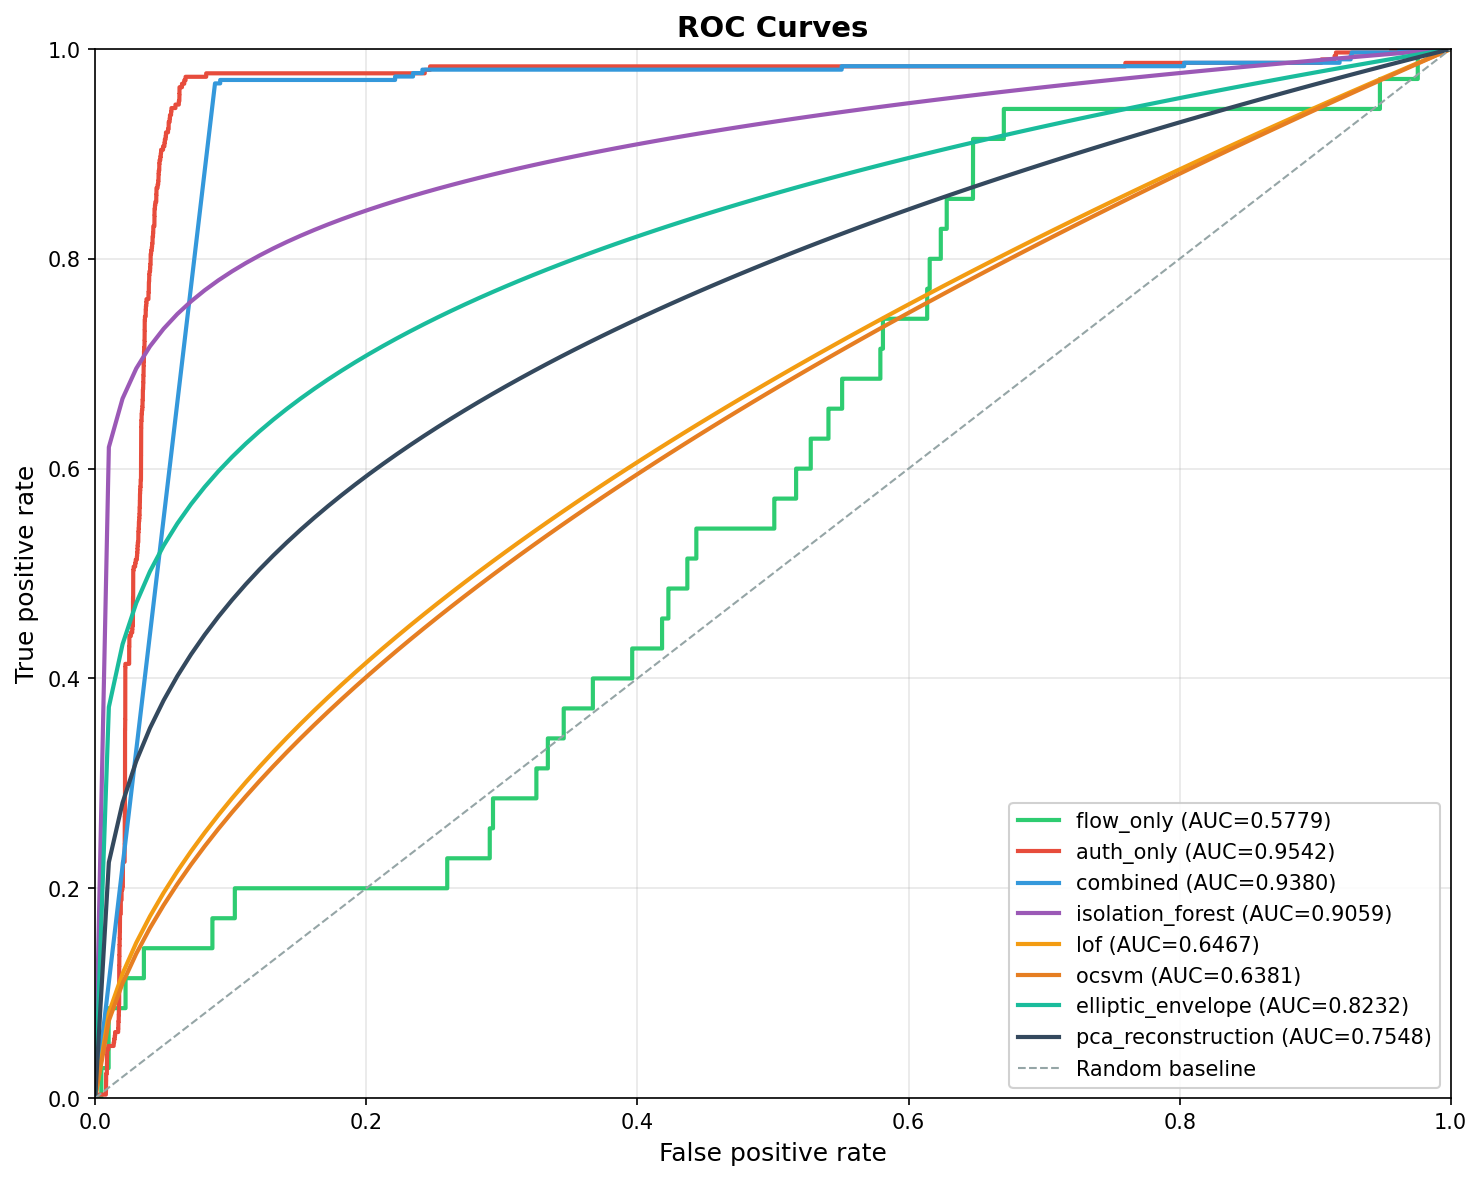
\includegraphics[width=0.95\columnwidth]{roc_curves.png}
\caption{ROC curves for all detection methods on LANL-2015. Auth-only achieves the highest AUC (0.9542), followed by combined (0.9380) and flow-only (0.5779). The auth-only and combined curves bow above the random baseline, demonstrating strong edge-level discriminative power. \textit{(Figure by: Wesley Gunawan)}}
\label{fig:roc}
\end{figure}

This figure validates the paper's central hypothesis that authentication logs provide the strongest signal for lateral movement detection, and that combining them with flow logs maintains high discriminative power while adding complementary coverage. The auth-only AUC of 0.9542 indicates that the scoring function (Equation~1) effectively ranks NTLM-based pass-the-hash attacks and network logon events above normal authentication traffic. The combined method's slightly lower AUC (0.9380) reflects the dilution effect of adding 131K flow edges to 409K auth edges, even with the 1.5$\times$ auth weight multiplier. The flow-only AUC of 0.5779 confirms that network flow patterns alone are nearly random for this detection task. Together, these results demonstrate that the unified graph approach preserves the strong signal from authentication logs while enabling path-based analysis that neither source can achieve alone.

Figure~\ref{fig:scores} shows the distribution of anomaly scores for all edges in the combined method. The baseline edges (green) are spread broadly across the score range from 0.0 to 0.9, with a large spike at 1.0 caused by the path boost mechanism that amplifies scores for edges appearing in suspicious multi-hop paths. The red-team edges (orange, barely visible due to their small count relative to 512K baseline edges) are concentrated near the high-score end of the distribution.

\begin{figure}[htbp]
\centering
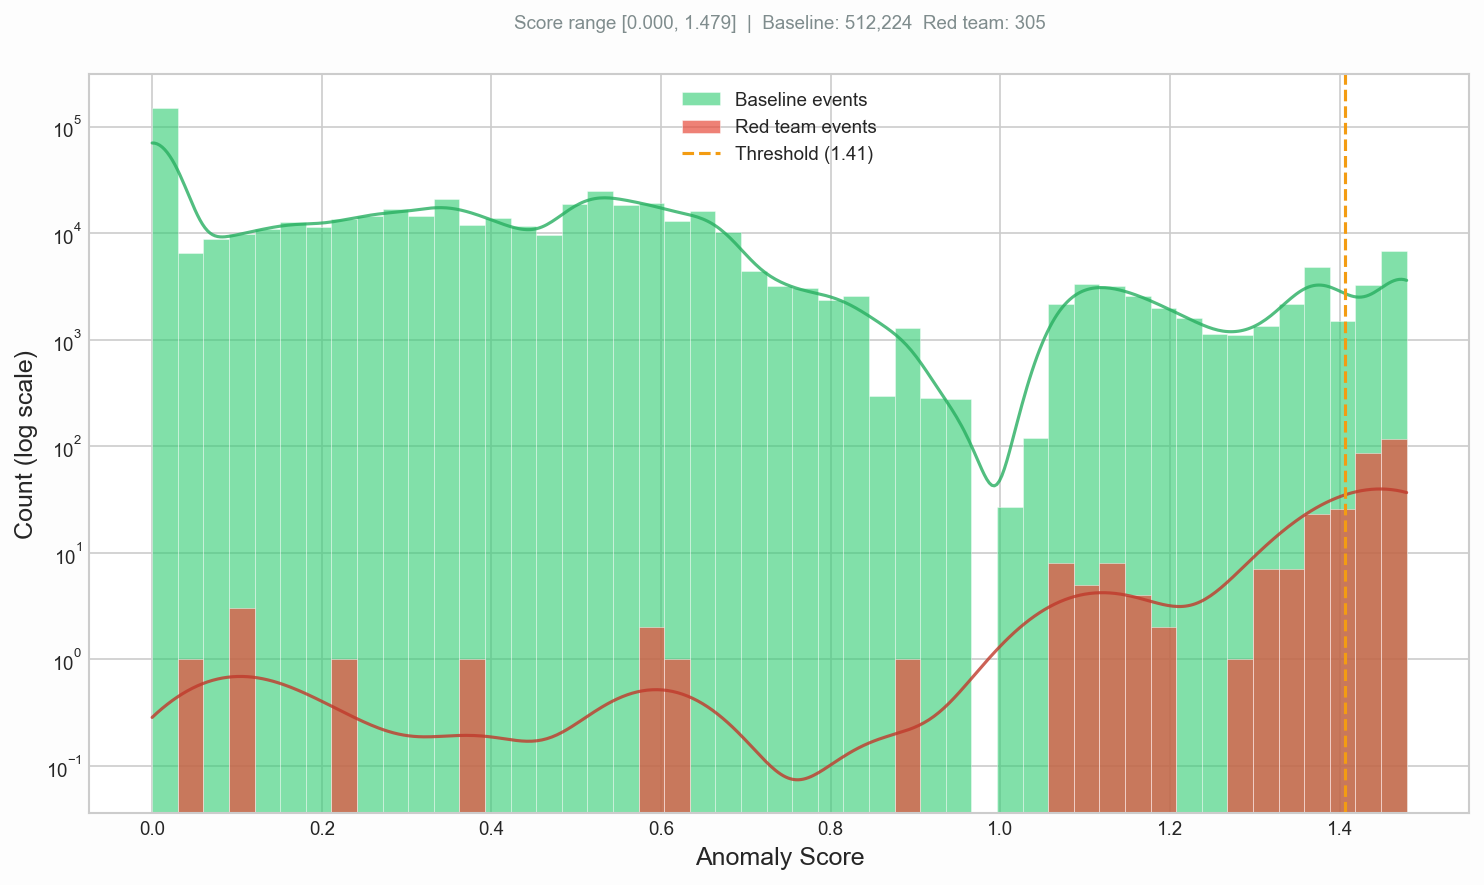
\includegraphics[width=0.95\columnwidth]{score_distribution.png}
\caption{Anomaly score distribution for the combined method. Baseline edges (green) span the full score range with a spike at 1.0 from path boosting. Red-team edges (orange) are concentrated at high scores but are too few to be visible in the histogram. \textit{(Figure by: Ibrahim Pehlivan)}}
\label{fig:scores}
\end{figure}

This figure reveals a key challenge in lateral movement detection: the baseline score distribution is broad and overlapping, making it difficult to set a single threshold that cleanly separates attack edges from benign edges. The large spike at score 1.0 is an artifact of the path boost mechanism (Section~4.4), which adds $0.1 \times \text{path\_score}$ to edges appearing in top-50 suspicious paths. This boost creates a bimodal distribution where a small fraction of edges receive maximum scores. The red-team edges, while concentrated at higher scores, are too few (305 out of 512K edges) to form a visible peak in the histogram. This visual evidence confirms that the scoring function produces a wide range of scores for baseline traffic, and that the rarity of attack edges in massive enterprise graphs makes them difficult to isolate with a fixed threshold. Future work should explore adaptive per-node baselines or supervised learning to improve separation.

% \subsection{Tabular Baselines on LANL-2015}
% \label{sec:baselines_lanl}

% Table~\ref{tab:methods_lanl} reports all eight methods evaluated on
% the same LANL-2015 run: three graph-based variants using the
% manually-weighted scoring formulas, and five unsupervised tabular
% detectors using \texttt{scikit-learn} defaults trained on benign
% edges only. All eight methods are scored against the same 305
% red-team source-destination pairs.

% \begin{table}[h]
% \centering
% \begin{tabular}{lcccc}
% \hline
% Method & Recall & FPR & F1 & AUC \\
% \hline
% \multicolumn{5}{l}{\textit{Graph-based (pair space)}} \\
% combined              & 0.662 & 0.020 & 0.039 & \textbf{0.954} \\
% auth\_only            & 0.747 & 0.030 & 0.036 & 0.951 \\
% flow\_only            & 0.013 & 0.030 & 0.002 & 0.579 \\
% \hline
% \multicolumn{5}{l}{\textit{Unsupervised tabular baselines (edge space)}} \\
% Isolation Forest      & 0.741 & 0.050 & 0.024 & 0.940 \\
% Elliptic Envelope     & 0.000 & 0.050 & 0.000 & 0.774 \\
% One-Class SVM         & 0.492 & 0.098 & 0.008 & 0.706 \\
% PCA Reconstruction    & 0.033 & 0.050 & 0.001 & 0.667 \\
% Local Outlier Factor  & 0.207 & 0.045 & 0.008 & 0.493 \\
% \hline
% \end{tabular}
% \caption{All eight methods on LANL-2015 (run \texttt{20260502\_165755}, 364{,}802-edge feature matrix, 305 red-team pairs). Graph methods evaluate threshold-dependent metrics in pair space (deduplicated source-destination pairs); tabular baselines evaluate in edge space. AUC is comparable across both spaces.}
% \label{tab:methods_lanl}
% \end{table}

% The combined graph method is strongest overall (AUC 0.954). Among
% baselines, Isolation Forest leads (AUC 0.940), within 0.015 of
% combined and within 0.011 of auth-only. LOF underperforms on the
% full data because the feature matrix is dominated by binary
% indicators, which saturate the local-density signal LOF relies on.
% The graph method's edge over the best baseline is small in AUC but
% larger in false-positive rate



\section{Discussion and Limitations}
\begin{itemize}
\item Interpretation of expected findings: does combining log sources improve detection as hypothesized?
\item Limitations of datasets: LANL represents a single cloud VPC network over 58 days with red-team attacks that may not capture all real-world techniques; DAPT2020 is a simulated environment that may not reflect full cloud VPC network complexity
\item Limited attack diversity: red-team events focus on specific lateral movement techniques (SMB, SSH, credential reuse), does not include living-off-the-land or fileless approaches
\item Comparison with related work results: how does our approach compare to Hopper, Euler, Kitsune in terms of detection and false positive rates (acknowledging different datasets)
\item Real-world deployment considerations: scalability to larger cloud VPC networks, handling encrypted traffic, integration with existing SIEM systems, log storage costs
\end{itemize}

\section{Conclusion}
\begin{itemize}
\item Summary: presented a graph-based approach combining network flow logs and authentication logs for lateral movement detection in cloud VPC networks, evaluated on LANL-Dataset-2015 and DAPT2020
\item Key takeaways: combining log sources in a unified graph improves detection over single-source baselines; structural and temporal graph features capture lateral movement patterns that individual log analysis misses; TCP dominance, rising fan-out, and anomalous timing provide strong detection signals
\item Future work: test on additional real-world cloud VPC datasets, integrate with cloud-native security services, explore machine learning classifiers on graph features, investigate encrypted traffic analysis, extend to live detection deployments
\end{itemize}

{\footnotesize \bibliographystyle{acm}
\bibliography{sample}}

\end{document}
